\subsection{Reconnaissance d’image de vêtements }

\begin{frame}{Une base de données plus complexe}
    \begin{block}{Description}
        Images de taille $28 \times 28$ pixels en noir et blanc : \\
        \quad - 60 000 images pour l'entrainement. \\
        \quad - 10 000 autres pour la vérification.
    \end{block}
    \begin{columns}
        \begin{column}{0.5\textwidth}
            \begin{figure}
                \centering
                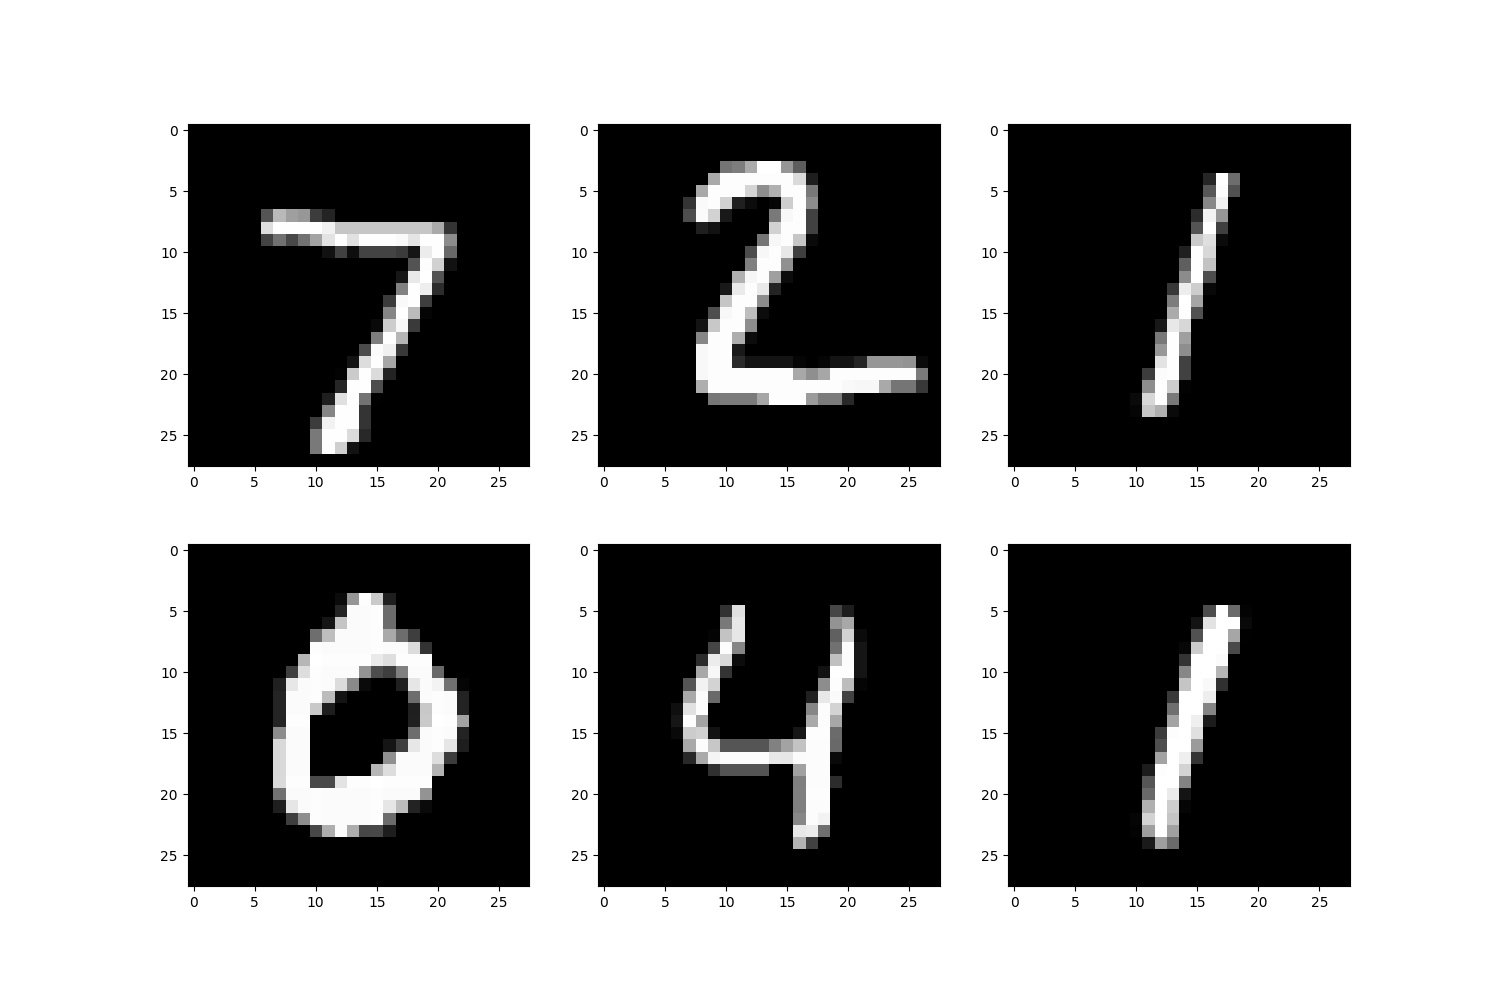
\includegraphics[width=\textwidth]{1-mnist.jpg}
                \caption{MNIST}
            \end{figure}
        \end{column}
        \begin{column}{0.5\textwidth}
            \begin{figure}
                \centering
                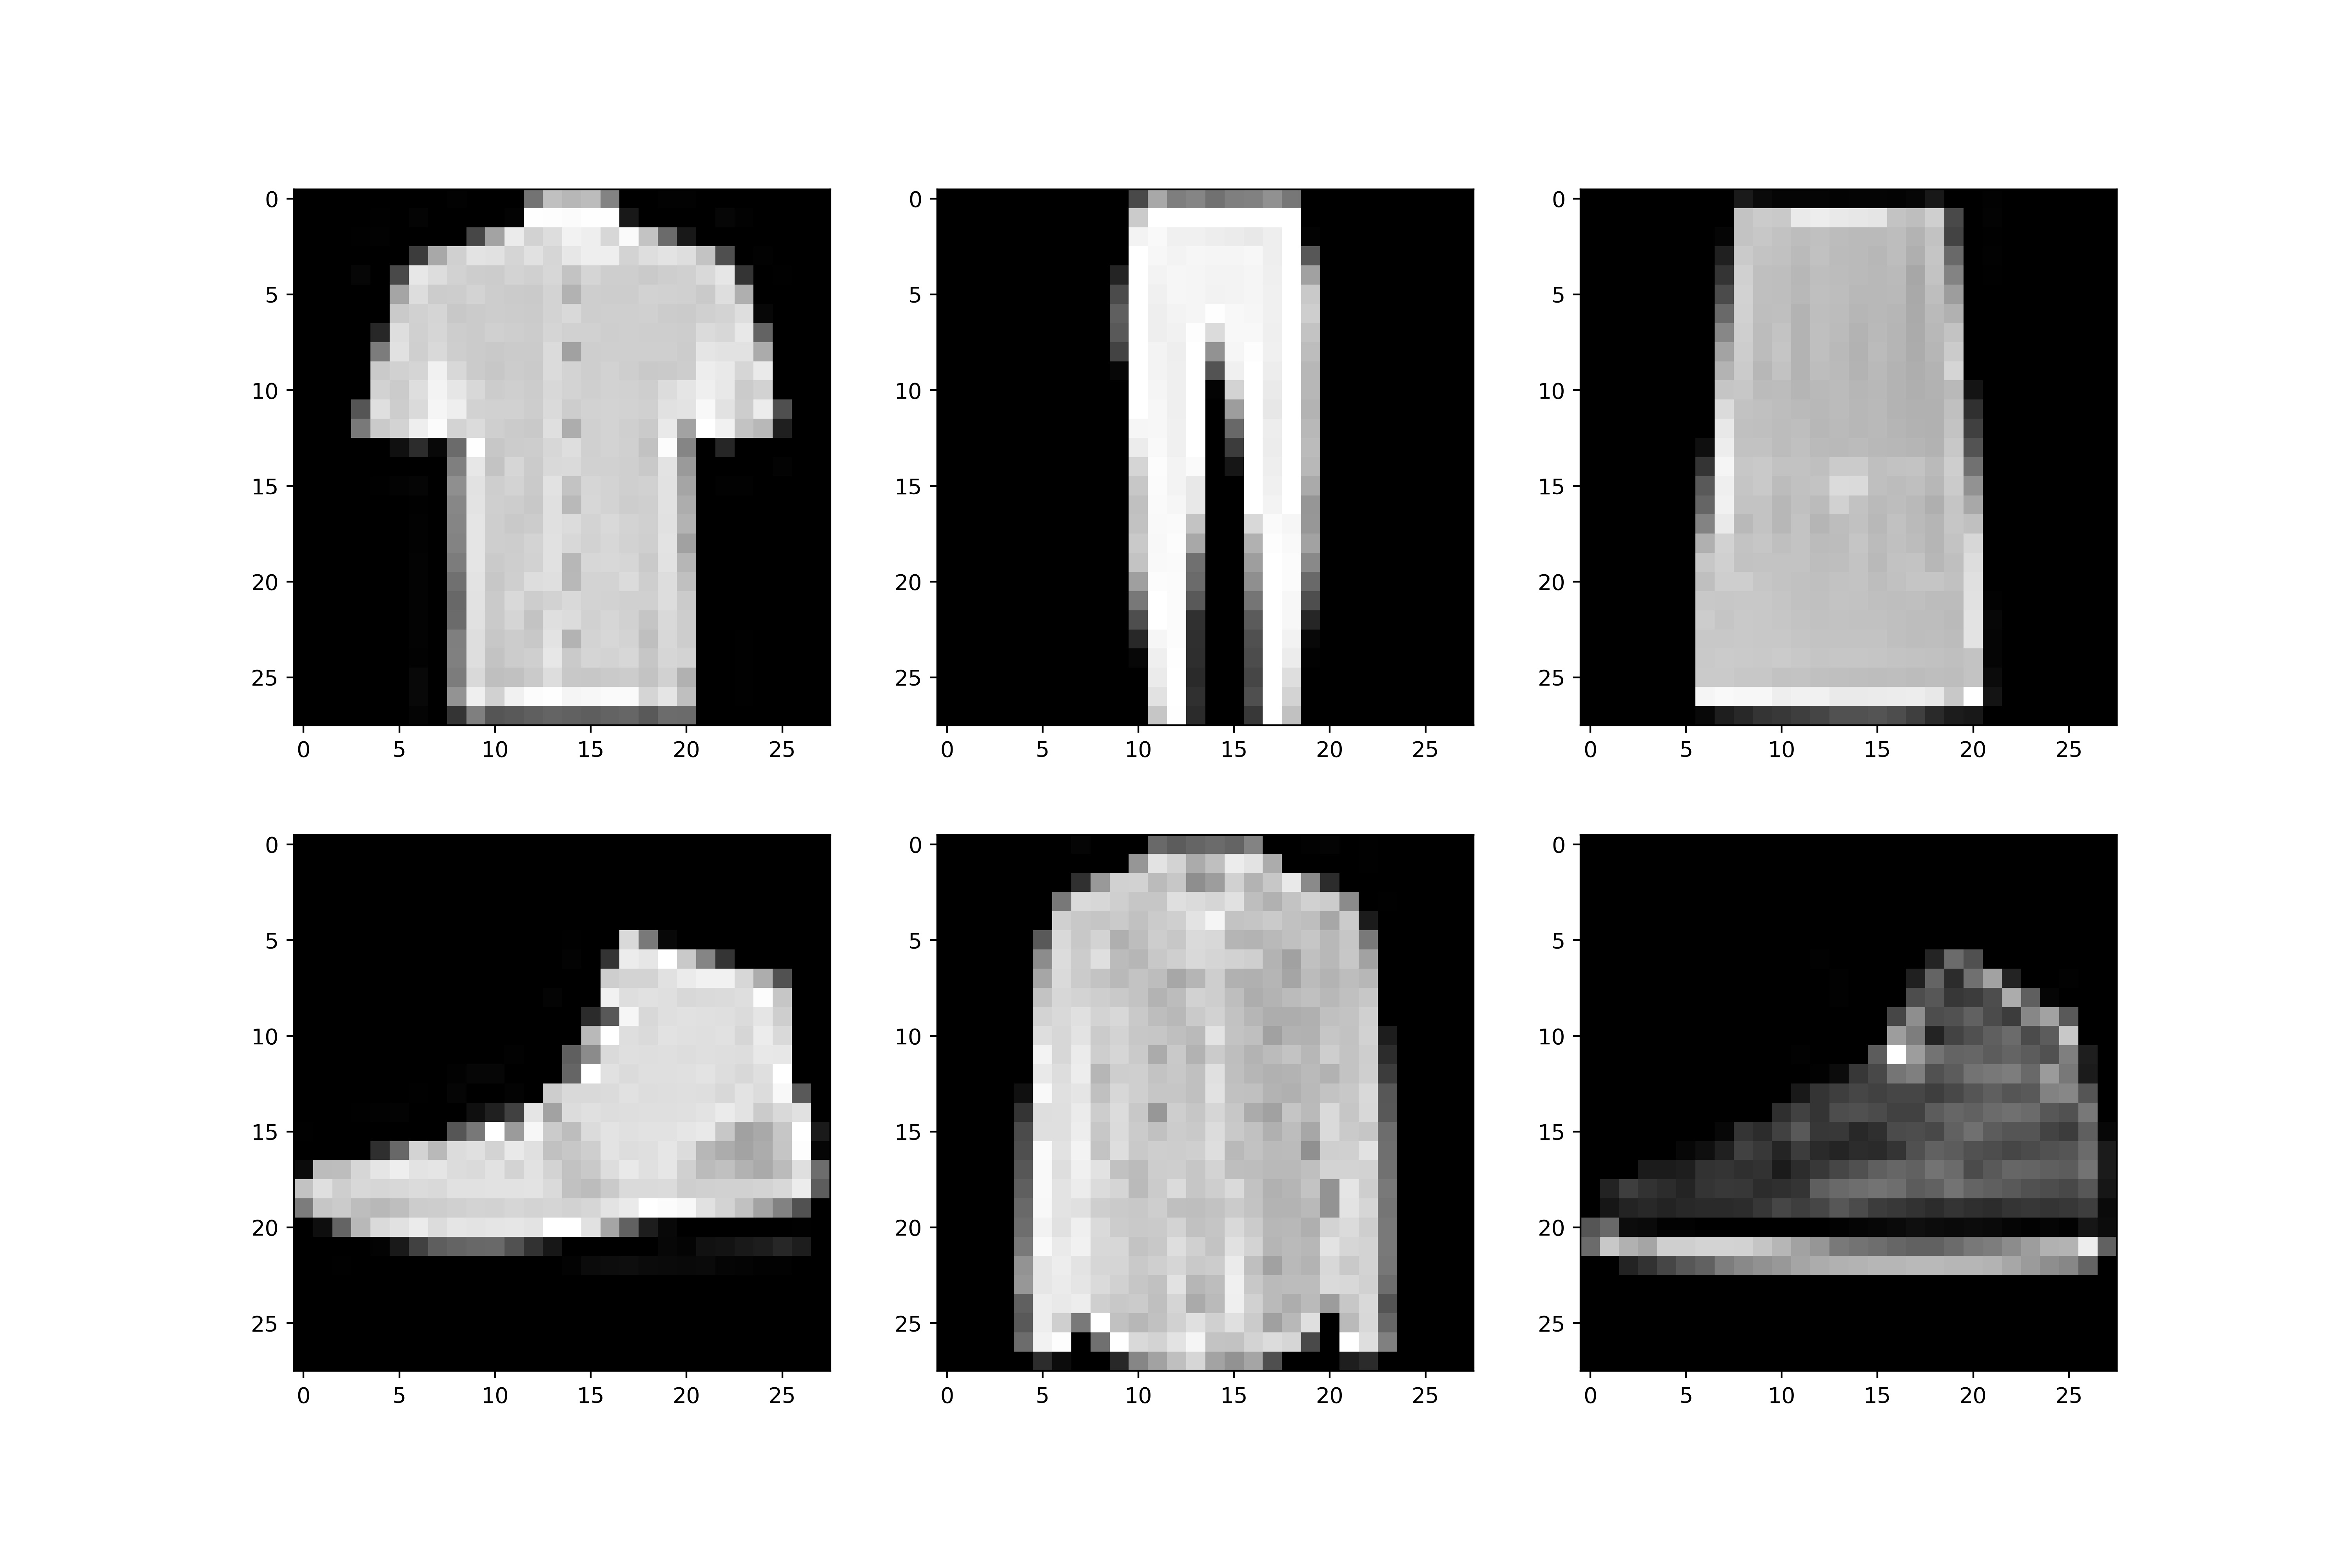
\includegraphics[width=\textwidth]{8-fashion-mnist.jpg}
                \caption{Fashion MNIST}
            \end{figure}
        \end{column}
    \end{columns}
\end{frame}

\begin{frame}{La convolution d'image}
    \begin{figure}
        \centering
        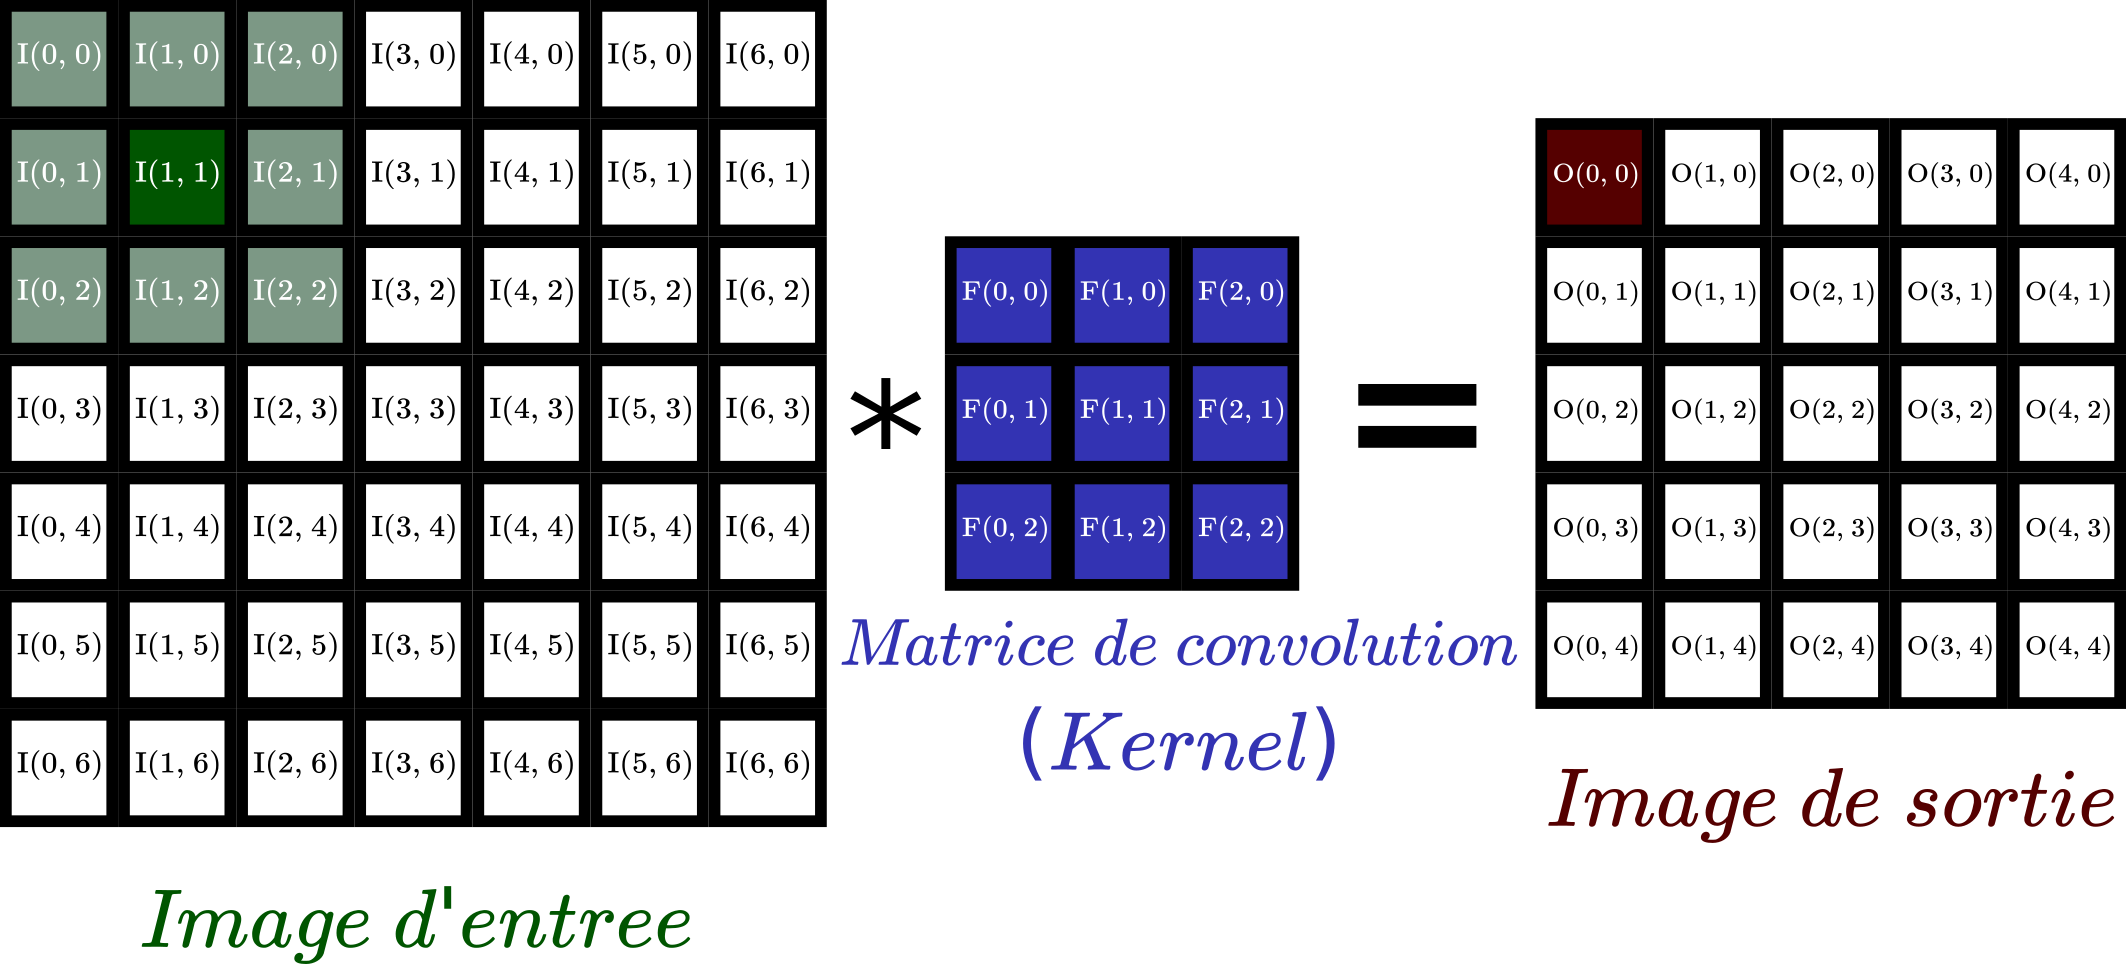
\includegraphics[width=\textwidth]{5-convolution.png}
        \centering
        \caption{Schéma de la convolution d'image $O(0, 0) = \sum_{i=0}^{2}\sum_{j=0}^{2}I(i, j)\times F(i, j)$}
    \end{figure}
\end{frame}


\begin{frame}{Un example de convolution d'image}
    \begin{columns}[T] % align columns
        \begin{column}{.6\textwidth}
            \begin{figure}
                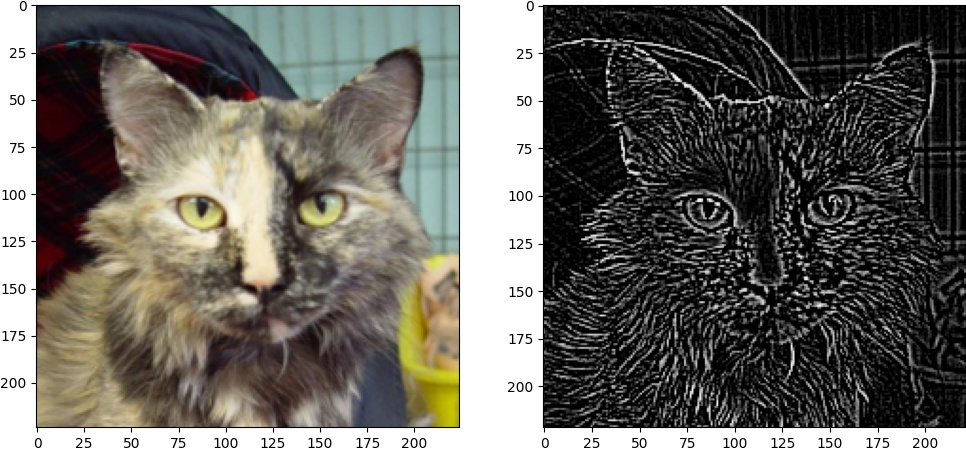
\includegraphics[width=\textwidth]{6-cat.jpg}
                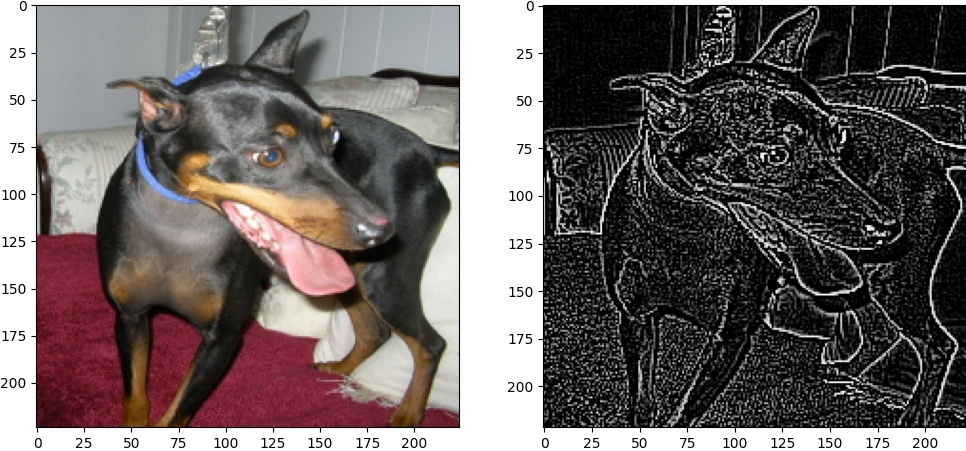
\includegraphics[width=\textwidth]{6-dog.jpg}
                \caption[]{Example de convolution d'image}
            \end{figure}
        \end{column}
        \begin{column}{0.35\textwidth}
            \begin{exampleblock}{Détection de contour}
                \begin{center}
                    \centering
                    $
                        F =
                        \begin{pmatrix}
                            -1 & -1 & -1 \\
                            -1 & 8  & -1 \\
                            -1 & -1 & -1
                        \end{pmatrix}
                    $
                \end{center}
            \end{exampleblock}
        \end{column}
    \end{columns}
\end{frame}


\begin{frame}{Le schéma du réseau de neurones convolutif}
    \begin{figure}
        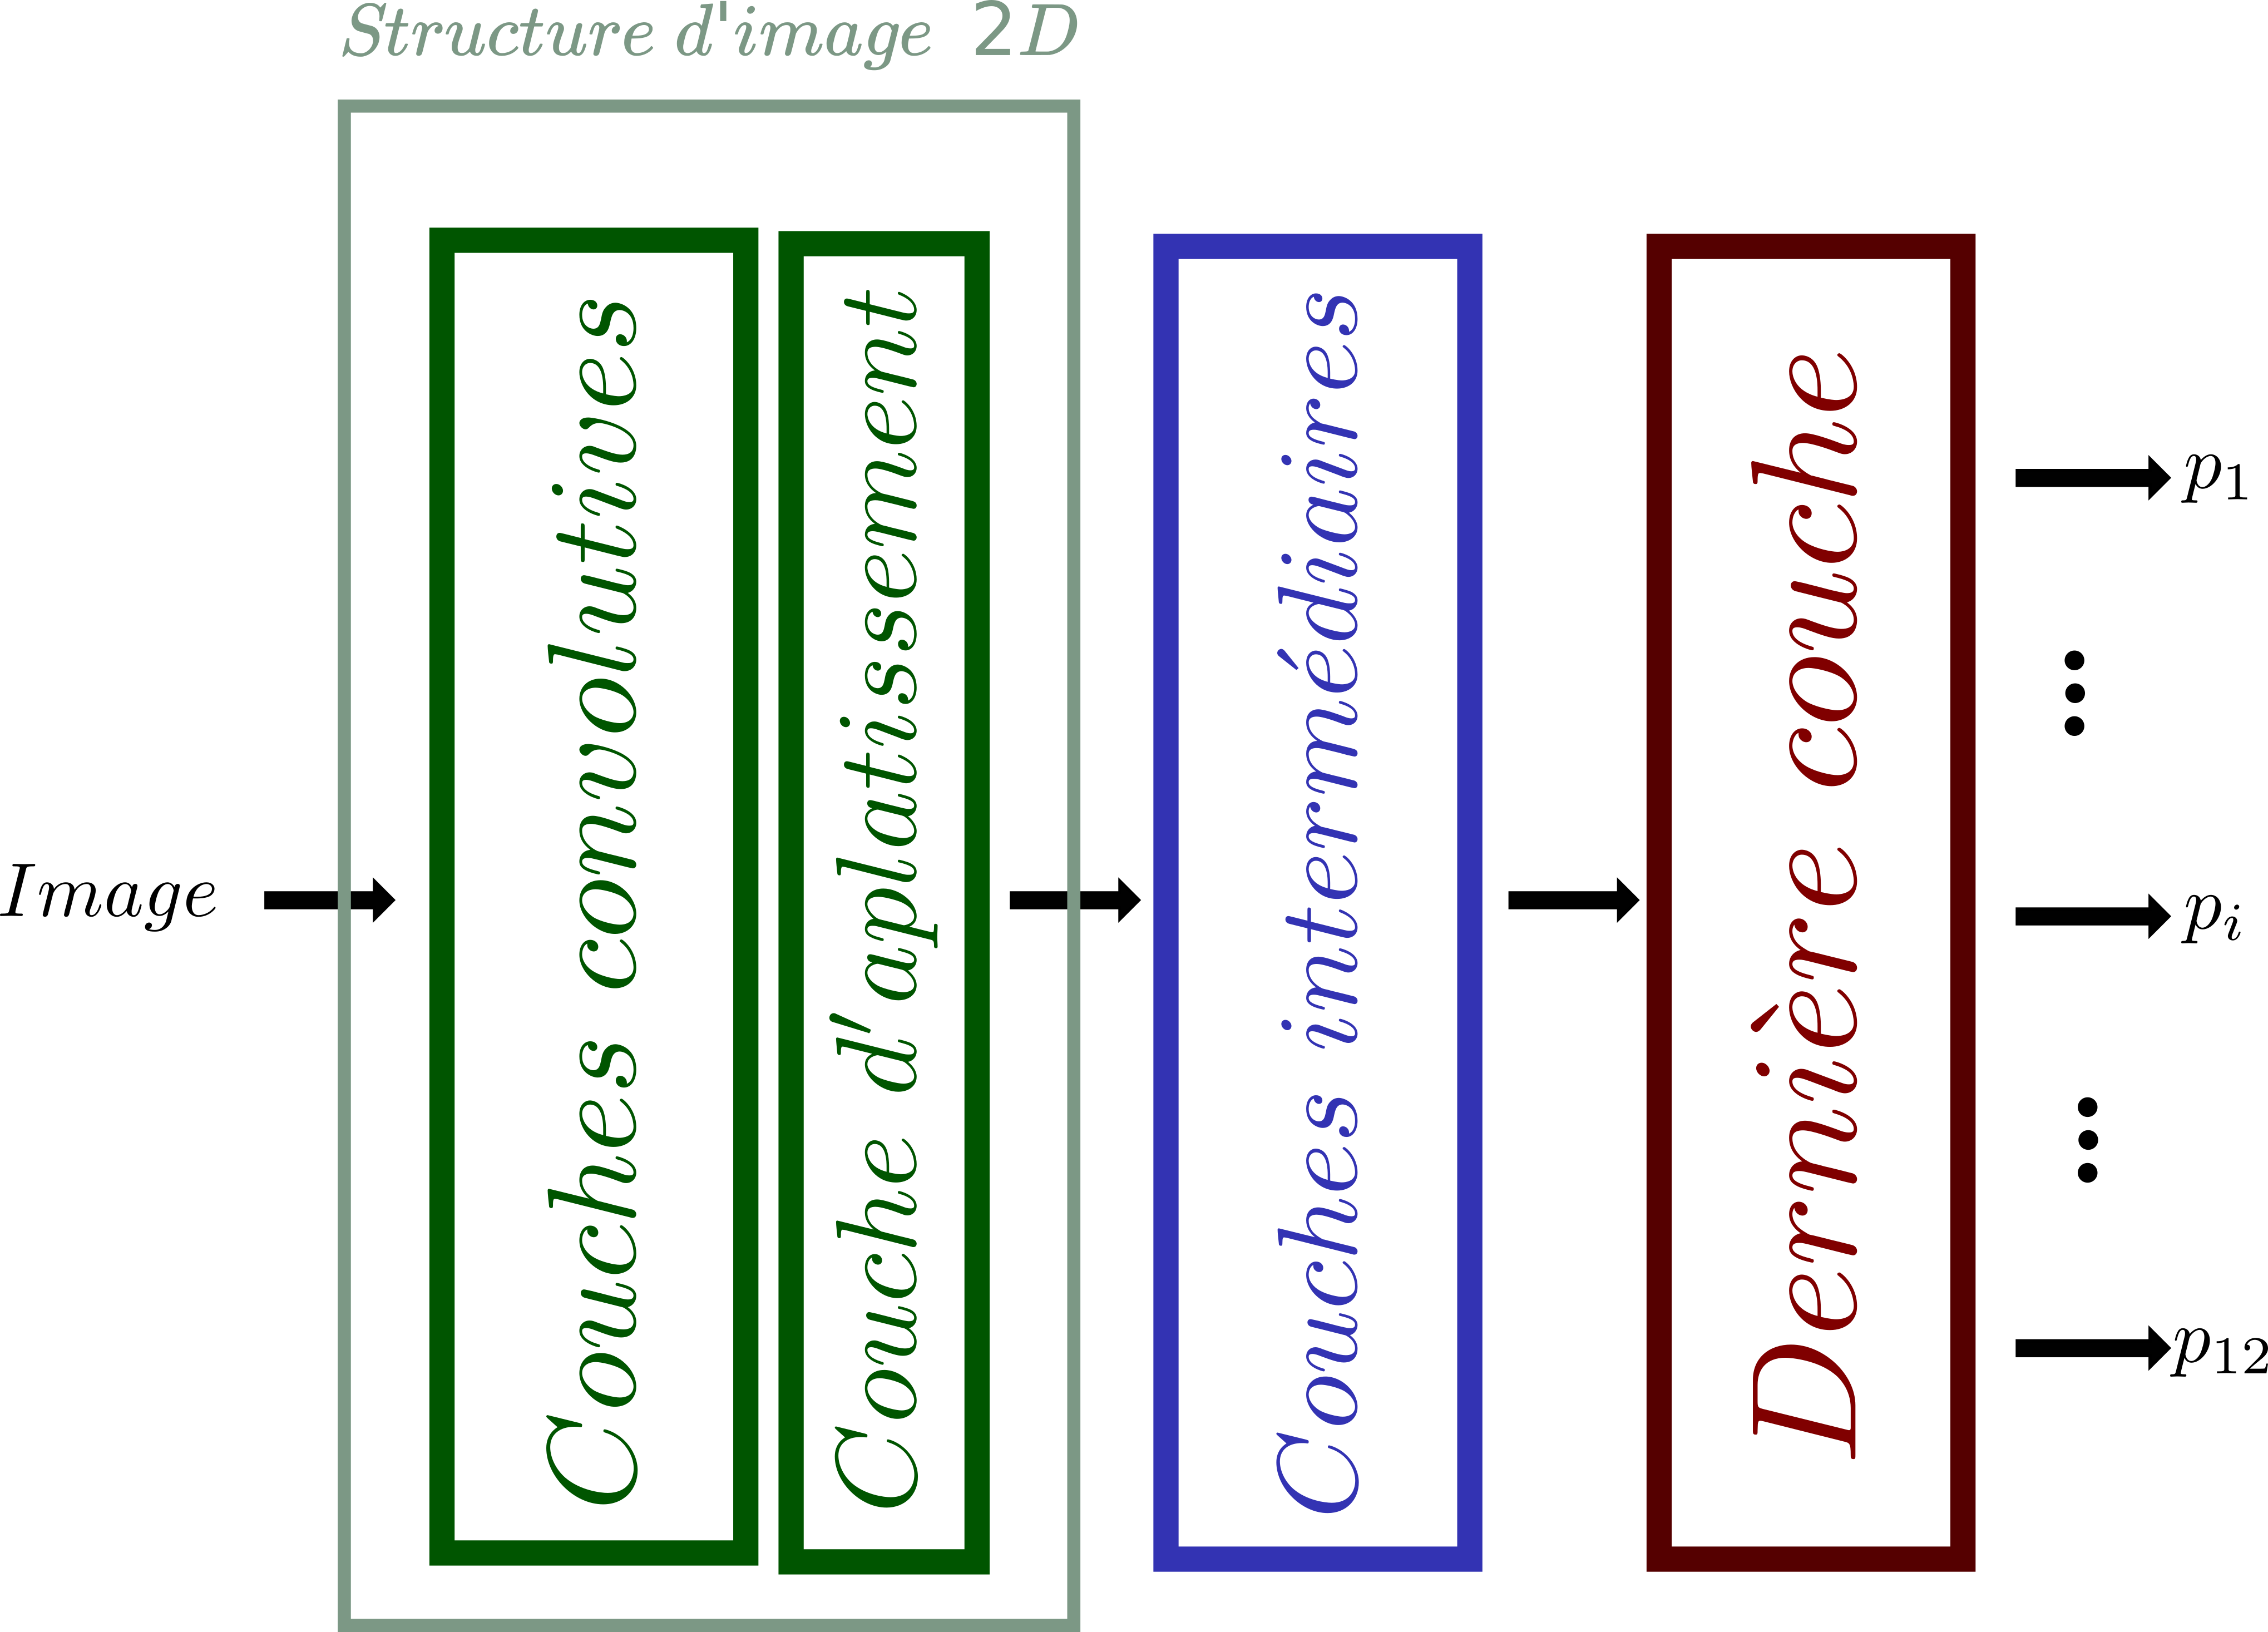
\includegraphics[height=0.7\textheight]{9-reseau convolutif.png}
        \caption[]{Schéma de réseau de neurones convolutif}
    \end{figure}
\end{frame}

\begin{frame}{Mes résultats}
    \begin{columns}[T]
        \begin{column}{.68\textwidth}
            \begin{figure}
                \centering
                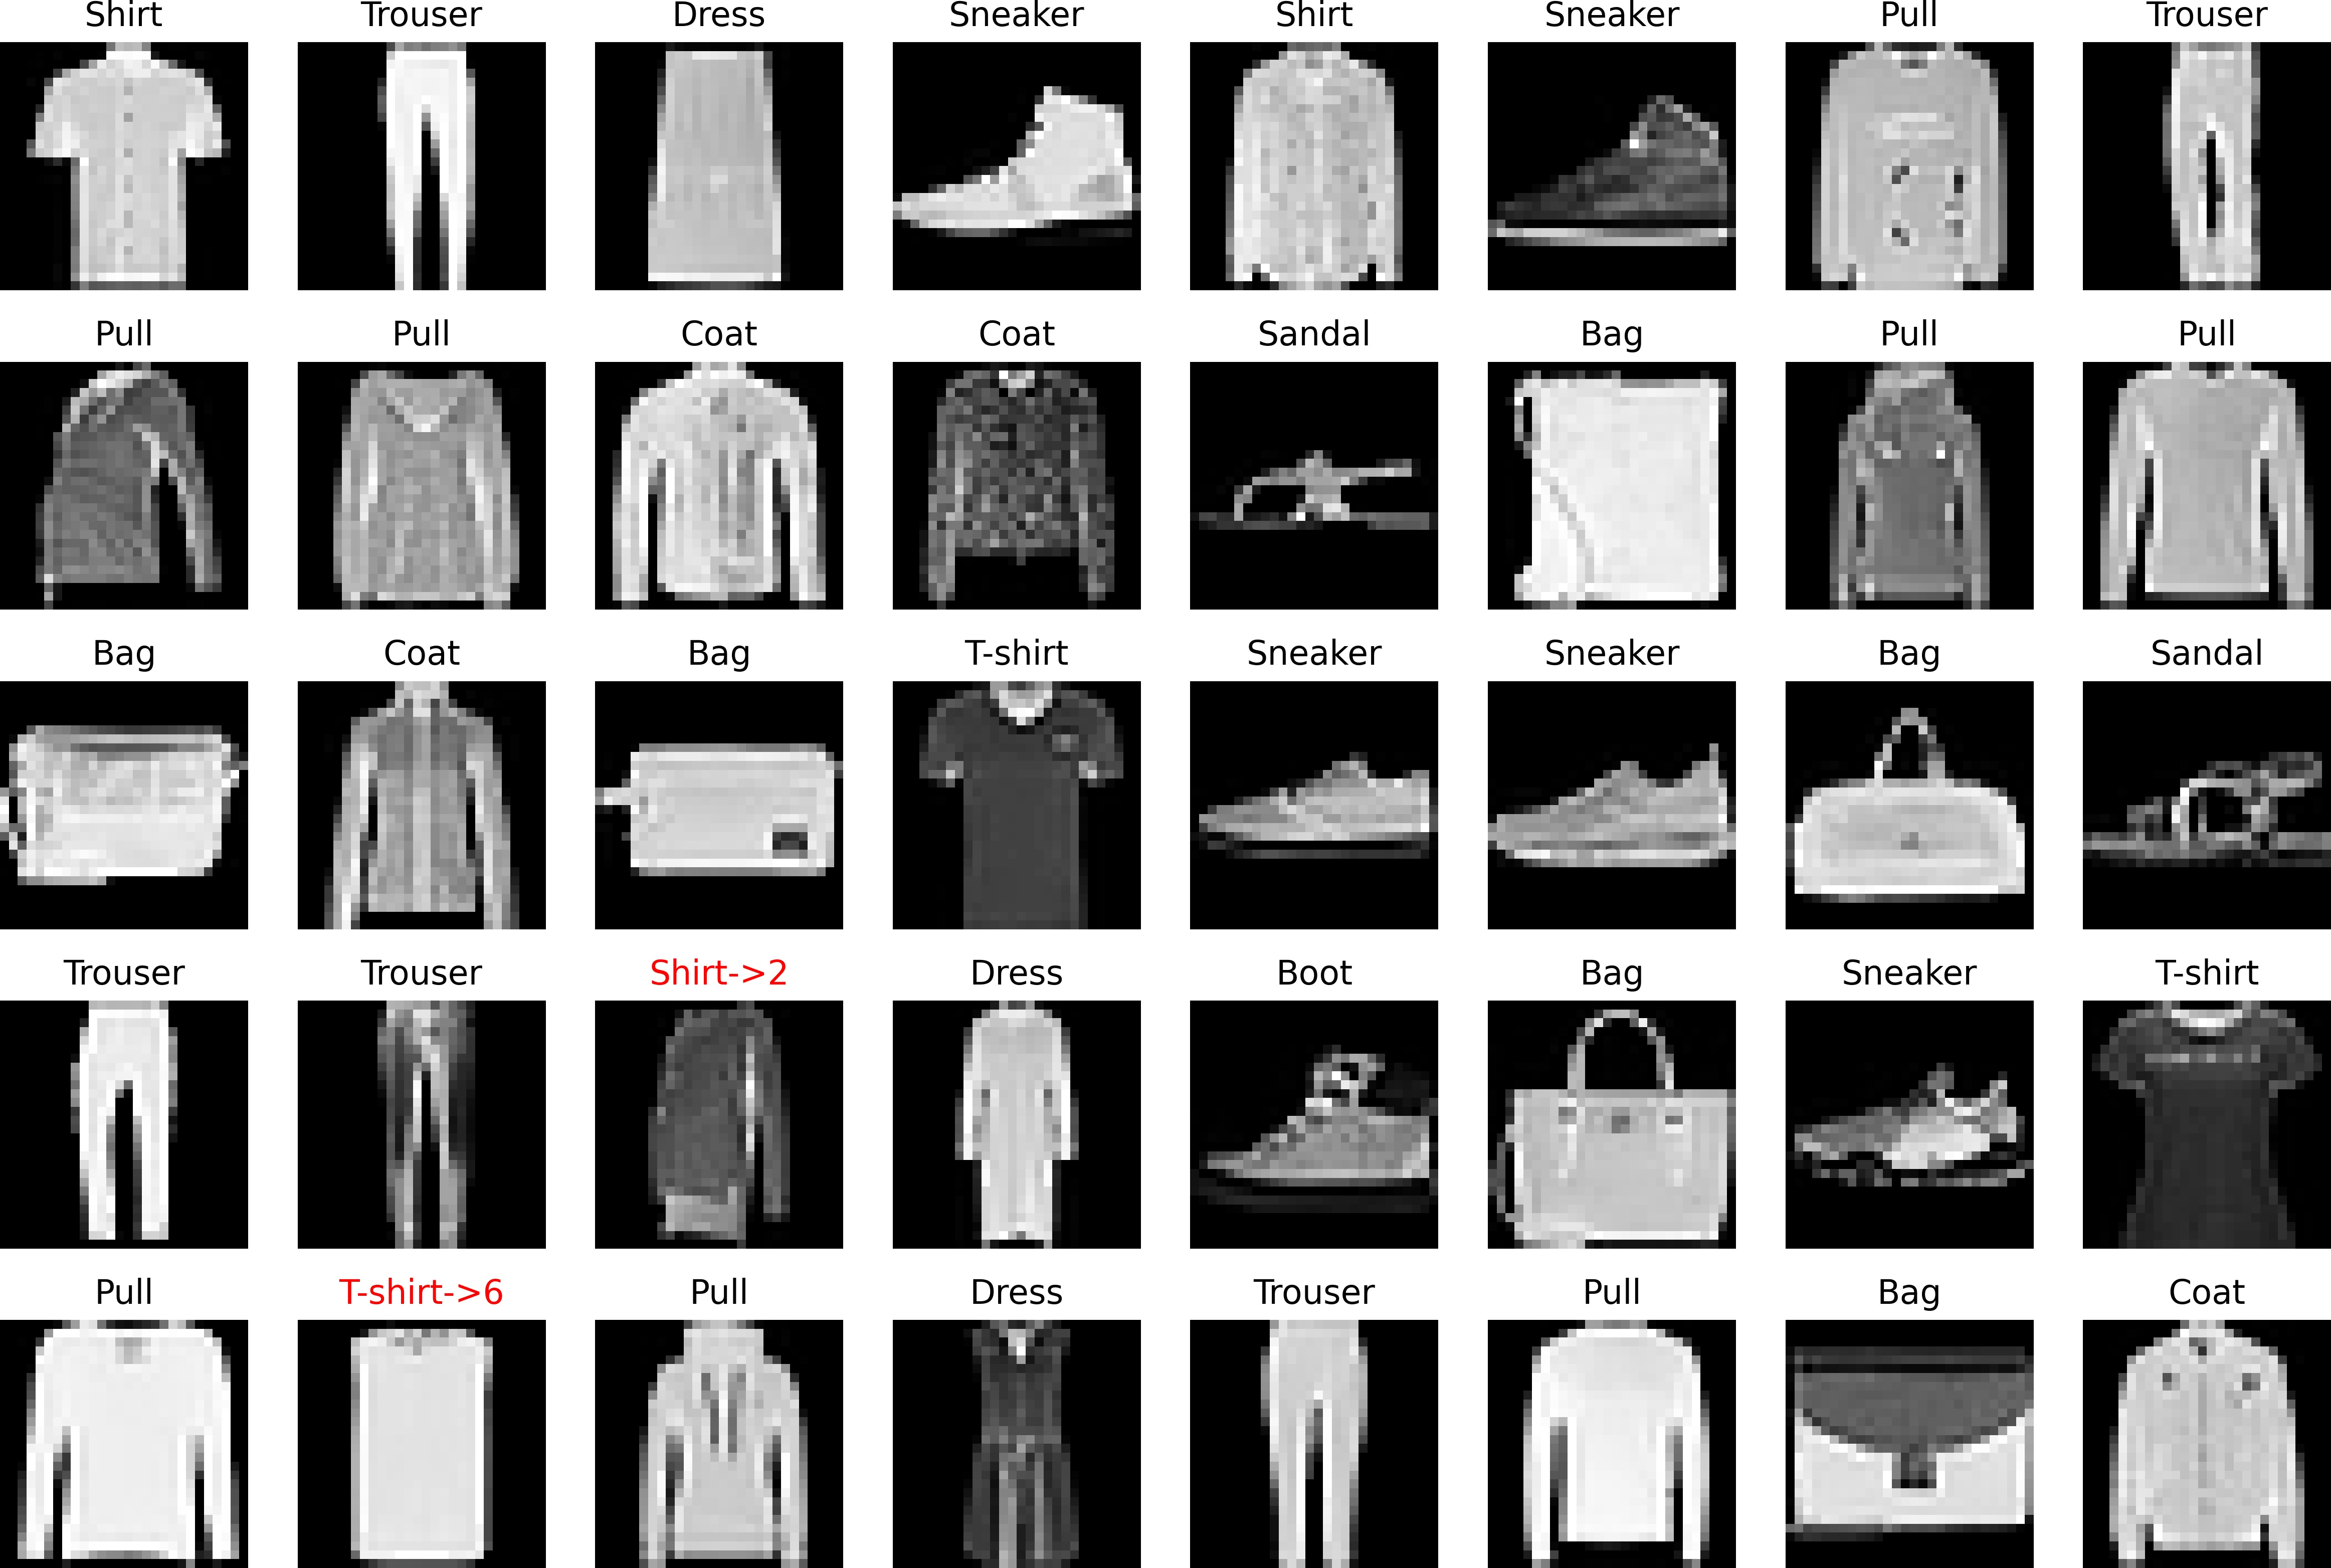
\includegraphics[width=\textwidth]{7-Resultat.jpg}
                \caption{Exemple sur un échantillon de 40 images $Fashion\ MNIST$}
            \end{figure}
        \end{column}
        \hfill
        \begin{column}{.35\textwidth}
            \bigskip	\bigskip	\bigskip
            \lstinputlisting[language=Python, firstline=15]{6-fashionDico.py}
        \end{column}
    \end{columns}
\end{frame}
